\documentclass{article}
\usepackage{graphicx}
\usepackage{listings}
\usepackage{amsmath}
\begin{document}

\section{Using Figure 2.4 as a model, illustrate the operation of merge sort on the array A=(3,41,52,26,38,57,9,49).}
\begin{figure}[!htb] 
  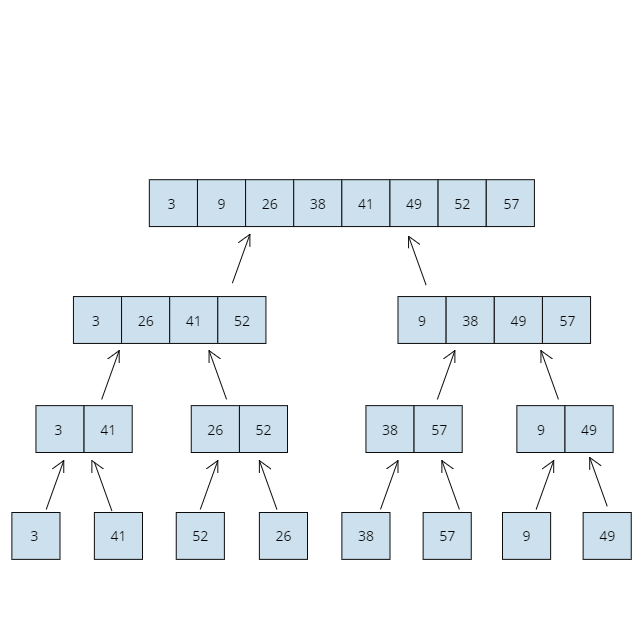
\includegraphics[width=\textwidth]{2_3-1.png}
\end{figure}


\section{Rewrite the Merge grocedure so that it does not use sentinels? instead stopping pnce either array L or Rhas had all elements copied back to A and then colying the remainder of the other array back into A}
\lstinputlisting[language=Python]{2.3-2/merge-sort.py}

\section{2.3-3}
Use mathematical induction to show that when $n$ is an exact power of 2, the solution of the recurrence

$T(n) = 
\begin{cases}
 2, & \mbox{if  $n= 2$} \\
 2T(n/2)+n, & \mbox{if $ n=2^k$, for $k > 1$} 
\end{cases}$ 

is $ T(n) = nlg(n)$

For $n=2$:
$T(2)=2=2lg(2)=nlg(n)$

For $n=4$:
$T(4)=2T(2)+4=2*2lg(2)+4*1=4*lg(2)+4*lg(2)=4*lg(4)=nlg(n)$

Assume, that for all $n \le k$ T(n)=nlg(n).
For $n = k*2$: $T(k*2)=2T(k*2/2)+ 2k=2k*lg(k)+2k=2k*lg(k) +2k*lg2=2k*(lgk + lg2)=2k*lg(2k)$

\section{2.3-4}
We can express insertion sort as a recursive procedure as follows. In order to sort A[1..n], we recursively sort A[1..n-1] and than insert A[n] into the sorted array A[1..n-1]. Write a recurrence for the worst-case running time of this recursive version of insertion sort.

$T(n) = 
\begin{cases}
 \Theta(1), & \mbox{if  $n= 1$} \\
 T(n-1)+n-1, & \mbox{if $n > 1$} 
\end{cases}$ 

\section{2.3-5}
Reffering back to the searching problem (see Exercise 2.1-3), observe that if the sequence A is sorted, we can check the midpoint of the sequence against v and eliminate half of the sequence from futher consideration. The binary search algorithm repeats this procedure, halving the size of the remaining portion of the sequence each time. Write pseudocode, either iterative or recursive? for binary search. Argue that the worst-case running time of binary search is $\Theta(lg(n))$

\lstinputlisting[language=Python]{2.3-5/binary-search.py}

Recurrence:
$T(n) = 
\begin{cases}
1, & \mbox{if  $n= 1$} \\
 T(n/2)+1, & \mbox{if $ n > 1$} 
\end{cases}$ 
 
let $n = 2^k$:

$n=1$: $T(1) = 1 = 1 + lg(0) = \Theta(lg(n)+ 1)$
$n=2$: $T(2) = T(1)+ 1 =  lg(1) + 1 +  1 = lg(1) + lg(2) = lg(2) = \Theta(lg(n))$
$n=k*2$: $T(2k)=T(k) + 1 = lg(k) + lg(2) = lg(2K)= \Theta(lg(n))$

\section{2.3-6}
Observe that the while loop of lines 5-7 of the Insertion sort procedure in Section2.1 uses a linear search to scan (backwards) through the sorted subarray A[1..j-1]. Can we use a binary search (see Exercise 2.3-5) instead to improve the overall worst-case running time of insertion sort $\Theta(n*lg(n))$

\lstinputlisting[language=Python]{2.3-6/insertion-sort-modified.py}

If we use List structure for a storage, insertion and deleting take $\Theta(1)$, so $T(n)= \Theta(n*lg(n))$
For Array structure there are still series of swaps required, so  so $T(n)= \Theta(n^2)$ 

\section{2.3-7}
Describe a $\Theta(nlg(n))$-time algorithm that, given a set S of n integers and another integer $x$, determines whether or not there exist two elements in S whose sum is exactly $x$.
\lstinputlisting[language=Python]{2.3-7/two-number-sum.py}


\end{document}